%%%%%%%%%%%%%%%%%%%%%%%%%%%%%%%%%%%%%%%%%%%%%%%%%%%%%%%%%%%%%%%%%%%%%
%% This is a (brief) model paper using the achemso class
%% The document class accepts keyval options, which should include
%% the target journal and optionally the manuscript type. 
%%%%%%%%%%%%%%%%%%%%%%%%%%%%%%%%%%%%%%%%%%%%%%%%%%%%%%%%%%%%%%%%%%%%%
\documentclass[journal=jacsat,manuscript=article]{achemso}

%%%%%%%%%%%%%%%%%%%%%%%%%%%%%%%%%%%%%%%%%%%%%%%%%%%%%%%%%%%%%%%%%%%%%
%% Place any additional packages needed here.  Only include packages
%% which are essential, to avoid problems later. Do NOT use any
%% packages which require e-TeX (for example etoolbox): the e-TeX
%% extensions are not currently available on the ACS conversion
%% servers.
%%%%%%%%%%%%%%%%%%%%%%%%%%%%%%%%%%%%%%%%%%%%%%%%%%%%%%%%%%%%%%%%%%%%%
\usepackage[version=3]{mhchem} % Formula subscripts using \ce{}
\usepackage{comment}

%%%%%%%%%%%%%%%%%%%%%%%%%%%%%%%%%%%%%%%%%%%%%%%%%%%%%%%%%%%%%%%%%%%%%
%% If issues arise when submitting your manuscript, you may want to
%% un-comment the next line.  This provides information on the
%% version of every file you have used.
%%%%%%%%%%%%%%%%%%%%%%%%%%%%%%%%%%%%%%%%%%%%%%%%%%%%%%%%%%%%%%%%%%%%%
%%\listfiles

%%%%%%%%%%%%%%%%%%%%%%%%%%%%%%%%%%%%%%%%%%%%%%%%%%%%%%%%%%%%%%%%%%%%%
%% Place any additional macros here.  Please use \newcommand* where
%% possible, and avoid layout-changing macros (which are not used
%% when typesetting).
%%%%%%%%%%%%%%%%%%%%%%%%%%%%%%%%%%%%%%%%%%%%%%%%%%%%%%%%%%%%%%%%%%%%%
\newcommand*\mycommand[1]{\texttt{\emph{#1}}}

%%%%%%%%%%%%%%%%%%%%%%%%%%%%%%%%%%%%%%%%%%%%%%%%%%%%%%%%%%%%%%%%%%%%%
%% Meta-data block
%% ---------------
%% Each author should be given as a separate \author command.
%%
%% Corresponding authors should have an e-mail given after the author
%% name as an \email command. Phone and fax numbers can be given
%% using \phone and \fax, respectively; this information is optional.
%%
%% The affiliation of authors is given after the authors; each
%% \affiliation command applies to all preceding authors not already
%% assigned an affiliation.
%%
%% The affiliation takes an option argument for the short name.  This
%% will typically be something like "University of Somewhere".
%%
%% The \altaffiliation macro should be used for new address, etc.
%% On the other hand, \alsoaffiliation is used on a per author basis
%% when authors are associated with multiple institutions.
%%%%%%%%%%%%%%%%%%%%%%%%%%%%%%%%%%%%%%%%%%%%%%%%%%%%%%%%%%%%%%%%%%%%%

\author{Nicholas A. Tiwari}
\affiliation[Carnegie Mellon University]
{Carnegie Mellon University, Pittsburgh, PA}
\author{Ashley J. Bird}
\affiliation[Lawrence Berkeley National Lab]
{Lawrence Berkeley National Lab, Berkeley, CA}
\author{Scott Blackburn}
\author{Andrew M. Park}
\affiliation[Chemours]
{The Chemours Company, Newark, DE}
\author{Ahmet Kusoglu}
\affiliation[Lawrence Berkeley National Lab]
{Lawrence Berkeley National Lab, Berkeley, CA}
\author{Shawn Litster}
\author{Zachary W. Ulissi}
\author{Gerald J. Wang}
\email{gjwang@cmu.edu}
\affiliation[Carnegie Mellon University]
{Carnegie Mellon University, Pittsburgh, PA}

\usepackage{booktabs}

%%%%%%%%%%%%%%%%%%%%%%%%%%%%%%%%%%%%%%%%%%%%%%%%%%%%%%%%%%%%%%%%%%%%%
%% The document title should be given as usual. Some journals require
%% a running title from the author: this should be supplied as an
%% optional argument to \title.
%%%%%%%%%%%%%%%%%%%%%%%%%%%%%%%%%%%%%%%%%%%%%%%%%%%%%%%%%%%%%%%%%%%%%
\title[An \textsf{achemso} demo]
  {Effects of Ionomer Backbone Composition on Morphology and O$_2$ Transport}

%%%%%%%%%%%%%%%%%%%%%%%%%%%%%%%%%%%%%%%%%%%%%%%%%%%%%%%%%%%%%%%%%%%%%
%% Some journals require a list of abbreviations or keywords to be
%% supplied. These should be set up here, and will be printed after
%% the title and author information, if needed.
%%%%%%%%%%%%%%%%%%%%%%%%%%%%%%%%%%%%%%%%%%%%%%%%%%%%%%%%%%%%%%%%%%%%%
\abbreviations{HOPI,PFSA}
\keywords{American Chemical Society, \LaTeX}

%%%%%%%%%%%%%%%%%%%%%%%%%%%%%%%%%%%%%%%%%%%%%%%%%%%%%%%%%%%%%%%%%%%%%
%% The manuscript does not need to include \maketitle, which is
%% executed automatically.
%%%%%%%%%%%%%%%%%%%%%%%%%%%%%%%%%%%%%%%%%%%%%%%%%%%%%%%%%%%%%%%%%%%%%
\begin{document}

%%%%%%%%%%%%%%%%%%%%%%%%%%%%%%%%%%%%%%%%%%%%%%%%%%%%%%%%%%%%%%%%%%%%%
%% The "tocentry" environment can be used to create an entry for the
%% graphical table of contents. It is given here as some journals
%% require that it is printed as part of the abstract page. It will
%% be automatically moved as appropriate.
%%%%%%%%%%%%%%%%%%%%%%%%%%%%%%%%%%%%%%%%%%%%%%%%%%%%%%%%%%%%%%%%%%%%%
\begin{tocentry}

\centering
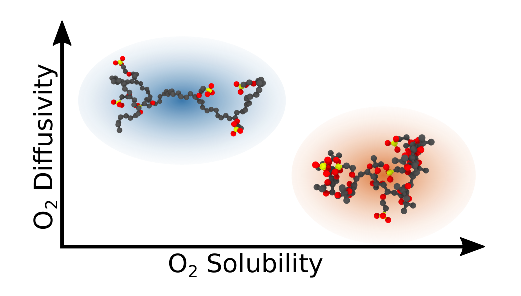
\includegraphics{tocfigure.eps}


\end{tocentry}

%%%%%%%%%%%%%%%%%%%%%%%%%%%%%%%%%%%%%%%%%%%%%%%%%%%%%%%%%%%%%%%%%%%%%
%% The abstract environment will automatically gobble the contents
%% if an abstract is not used by the target journal.
%%%%%%%%%%%%%%%%%%%%%%%%%%%%%%%%%%%%%%%%%%%%%%%%%%%%%%%%%%%%%%%%%%%%%
\begin{abstract}
Proton exchange membrane  (PEM) fuel cells are a compact and lightweight power source that use an acidic polymer membrane as an electrolyte. They have a lower carbon footprint than combustion engines and are not subject to the restrictively low gravimetric energy densities of modern batteries, making them ideal for heavy-duty transport applications such as trucks and buses. However, resistance to oxygen transport in the ion-conductive polymer, or ionomer, that coats catalyst particles in the cell cathode has been associated with decreased cell power output and durability. In this research, we employ molecular simulation techniques to compare the oxygen transport properties between an ionomer with a PTFE backbone, similar to commercial offerings, and a recently developed high oxygen permeability ionomer (HOPI) whose backbone is comprised of dioxolane rings. We find that oxygen permeability is up to four times higher in the HOPI, owing to substantially higher oxygen solubility. 
\end{abstract}

%%%%%%%%%%%%%%%%%%%%%%%%%%%%%%%%%%%%%%%%%%%%%%%%%%%%%%%%%%%%%%%%%%%%%
%% Start the main part of the manuscript here.
%%%%%%%%%%%%%%%%%%%%%%%%%%%%%%%%%%%%%%%%%%%%%%%%%%%%%%%%%%%%%%%%%%%%%
\section{Introduction}
Proton exchange membrane fuel cells (PEMFCs) are a promising power source for heavy-duty transportation due to their relatively low operating temperatures and high power density; however, several barriers prevent their widespread adoption\cite{Cullen2021, pemfc-costing}, including degradation of the platinum catalyst, which reduces the operating efficiency and increases the lifetime operating cost of a PEMFC \cite{weber_critical_2014,braaten_studying_2020, wood_nafion_2009,ferreira_instability_2005,braaten_contaminant_2019,yu_mechanism_2011}. Numerous strategies have been investigated to mitigate these weaknesses, including improving catalyst activity \cite{molmen_recent_2021,chandran_high-performance_2018,koh_effects_2008,he_single_2020} and developing better carbon supports \cite{ramaswamy_carbon_2020,yu_carbon-support_2009}. There has also been a considerable effort dedicated to modifying the ion-conductive polymer (ionomer), with the goal of improving gas permeability \cite{jomori_analysis_2012,Greszler_Caulk_Sinha_2012,sakai_analysis_2009,mohamed_effects_2009}. 

It is this last approach that motivates the present work, in which we investigate the relationship between ionomer morphology and oxygen permeability using molecular simulation. Ionomers used in PEMFCs are often perfluorosulfonic acid (PFSA) polymers composed of polytetrafluoroethylene (PTFE) backbones and sulfonate functionalized pendant side chains; commercially available examples of such ionomers include Nafion™, Flemion™, and Aciplex™. Such ionomers have been shown experimentally to form dense, crystalline domains in which the backbone segments are neatly stacked\cite{modestino_controlling_2012, ludvigsson_crystallinity_2000}, reducing the fractional free volume (FFV) of the ionomer, which in turn reduces gas permeability throughout the system. It has been shown that reducing the equivalent weight (polymer mass per ionic group) tends to lead to higher FFVs \cite{wang_evaluation_2012}, although there is evidence that proton transport is hindered at equivalent weights below 700 g/mol\cite{giffin_interplay_2013}. 

Longer side chains can also increase the free volume by reducing crystallinity; they are able to access more space in the polymer matrix, where they act as impurities, inhibiting the formation and growth of microcrystallites \cite{ghielmi_proton_2005}. However, the sulfonic groups that terminate side chains have a high affinity for the platinum catalyst, and the increased flexibility of longer side chains facilitates the adsorption of sulfonate moieties to the platinum \cite{kodama_effect_2018}. This results in a high density monolayer of sulfonates at the ionomer-platinum interface, which is difficult for O$_2$ to permeate. 

Substitution of PTFE backbone units with bulkier structures has a desirable effect on fractional free volume, oxygen transport and cell durability as well\cite{braaten_integration_2022,rolfi_new_2018,jinnouchi_role_2021}, and is the focus of this work. Amorphous fluoropolymers, first developed by DuPont in the 1980s under the Teflon\texttrademark AF trademark, are typically composed of tetrafluoroethylene and asymmetric dioxolane rings. The presence of rings inhibits chain packing, which prevents crystallite formation and results in high fractional free volume \cite{Resnick_Buck_2000} and improved gas permeability. The permeability of O$_2$ in Teflon\texttrademark AF2400 is orders of magnitude higher than in PTFE \cite{Alentiev_Shantarovich_Merkel_Bondar_Freeman_Yampolskii_2002, Merkel_Bondar_Nagai_Freeman_Yampolskii_1999}. 

Rolfi et al. and Katzenberg et al. are the first published works to propose and synthesize ionomers which incorporate dioxolane rings, similar to the ones present in amorphous fluoropolymers, into the ionomer backbone \cite{rolfi_new_2018,katzenberg_highly_2020}. In this work, we use MD simulations and small angle X-ray scattering (SAXS) experiments to evaluate differences in structure and transport properties between an ionomer with an amorphous backbone composed of dioxolane rings, called the high oxygen permeability ionomer (HOPI), and a sample PFSA chemistry, with a TFE backbone, which is representative of commercially available ionomers. The chemical structures are shown in Figure \ref{fig:chemcomp}. 

\begin{figure}[h!]
  \includegraphics[width=.9\linewidth]{visualizations.png}
  \centering
  \caption{Chemistries and visualizations for the sample PFSA and HOPI. $x$ is the number of backbone units per polymer repeat unit, and $z$ is the number of polymer repeat units. Red indicates oxygen, yellow indicates sulfur. Orange backbones indicate the HOPI, and blue backbones indicate PFSA. Fluorine occludes important geometric features, and so is not shown.}
\label{fig:chemcomp}
\end{figure}


\section{Motivation}
The permeability $P_x$ of a gas species $x$ in a polymeric membrane is given by the product of the gas's diffusion coefficient $D_x$ and solubility $S_x$ within that polymeric environment:

\begin{equation}
    \label{eqn:permeability}
    P_x = D_xS_x
\end{equation}

As such, there are two approaches to increasing permeability, either via the diffusivity or via the solubility. In practice, these approaches are not entirely independent, as reviewed extensively by Kusoglu and Weber\cite{Kusoglu2017} in the context of ionomers. Both quantities 

\section{Methods}

\subsection{Simulations}
In this research, two molecular dynamics models are developed and investigated. The first is a bulk model which contains exclusively water and ionomer, and is used for diffusivity and density calculations. The second is a thin film model that contains water, ionomer, and platinum and is used for solubility calculations. Initial configurations were generated using the Enhanced Monte Carlo (EMC) software package\cite{in_t_veld_temperature-dependent_2003}, and simulations were performed using LAMMPS \cite{thompson_lammps_2022}.

Equivalent weights were set to 993 g/mol and 852 g/mol for PFSA and HOPI, respectively. This corresponds to 7 backbone units and 2.33 backbone units per polymer repeat unit. All sulfonic groups were assumed to be ionized. Gas permeability in a membrane varies with external relative humidity (RH) \cite{broka_oxygen_1997,novitski_determination_2015,schalenbach_gas_2015}, so the number of water molecules in the model was manipulated to determine the effect of hydration on oxygen transport. Hydronium ions were added to offset the negative charge incurred by the deprotonated sulfonate groups and were counted towards the total number of waters.  The simulation water content ranged from 1 water per sulfonic group to 6.6 waters per sulfonic group; the minimum water content was chosen to be 1 because total ionization was assumed. These water contents correspond to ionomer water uptake at ambient relative humidities ranging from 53\% to 100\%. 

Visualizations of both systems are given in Figure \ref{fig:chemcomp}. Polymer-polymer interactions are described using the DREIDING force field \cite{mayo_dreiding_1990}, and polymer-platinum interactions are described using the force field proposed by Brunello et al. \cite{brunello_interactions_2016}. The simulations were run for 10 nanoseconds using a time step of 0.5 femtoseconds. The first nanosecond was a high temperature stage conducted at 1000 K to allow polymers to overcome kinetic barriers, the second nanosecond was an annealing stage where the temperature was reduced from 1000 K to 353 K, and the remaining time was an equilibration and data collection stage, which was conducted at 353 K. The next two sections provide detailed information on the methods used to develop bulk and thin-film models. 

\subsubsection{Bulk System}
Eight simulations, each starting from a different initial configuration, were performed at each humidity. The supercell for each simulation contained 20 polymer chains, 40 O$_2$ molecules, and a varying number of waters. The boundary conditions were periodic in all three dimensions. The supercells were initialized to a density of 1.6 g/cm$^3$, and the initial cell edge length ranged from 47 {\AA} to 50 {\AA}. The system was held in the NVT ensemble for the annealing and temperature reduction stages, and switched to the NPT ensemble with a pressure of 1 atm for the data collection stage. The mean squared displacement (MSD) data for O$_2$ were extracted from the final four nanoseconds of each simulation and used to calculate the O$_2$ self-diffusion coefficient at different water numbers. The self-diffusion coefficients were calculated by the Einstein relation, given in Equation \ref{eqn:einstein}. 

\begin{equation}
  \label{eqn:einstein}
  D_{O_2} = \frac{1}{6} \lim_{t \to \infty} \frac{d}{dt} \frac{1}{N} \sum_{i=1}^{N} \langle|r_{O_2}(t) - r_{O_2}(0)|\rangle^2 
\end{equation}

$D_{O_2}$, the oxygen self-diffusion coefficient, was calculated by fitting a linear model to mean squared displacement data, which is given by $\frac{1}{N} \sum_{i=1}^{N} \langle|r_{O_2}(t) - r_{O_2}(0)|\rangle^2 $ in Equation \ref{eqn:einstein}. The model was fitted using linear least squares regression. The bulk density was calculated by averaging the supercell density for the final four nanoseconds of the data collection stage. 
\subsubsection{Thin-film System}
A single NVT simulation was conducted at each humidity. Each supercell contained eight polymer chains, and a varying number of waters depending on the humidity. The liquid phase in each supercell was initialized to the bulk density at that humidity, and the system was assumed periodic only in the $x$ and $y$ directions. In the $z$ direction, the system was constrained by the platinum slab at the bottom of the box and a harmonic wall boundary condition at the top of the box. The functional form of the harmonic boundary condition is given in Equation \ref{eqn:harmonic}. 
\begin{equation}
    \label{eqn:harmonic}
    U = k(r-r_c)^2 \qquad r < r_c
\end{equation}

Where $U$ is the potential energy, $r$ is the distance from a particle to the boundary condition, $k$ is the spring constant, which was set to 600.0 kcal/mol, and $r_c$ is the cutoff distance, which was set to 4 angstroms below the top of the supercell. The platinum slab was immobilized to ensure that platinum atoms did not migrate out of the supercell during the simulation. The solubility of oxygen in the liquid phase was determined using the final nanosecond of each simulation, where it was assumed that the supercell was in chemical equilibrium with gas phase O$_2$. To calculate the solubility, we assumed that the supercell was in chemical equilibrium with an oxygen gas phase. This was achieved via the GCMC package in LAMMPS, which performs grand canonical Monte Carlo insertions with a fictitious ideal gas reservoir, as described by Frenkel and Smit \cite{frenkel_understanding_2002}. Solubility was determined by counting the number of O$_2$ molecules present in the supercell at the time steps where GCMC exchanges were attempted, and averaging this count over the whole GCMC run.

\subsection{Water Content Measurements}
Swelling experiments were conducted on ionomer thin films using environmental ellipsometry to establish ionomer water content as a function of relative humidity. Data are given in Figure \ref{fig:water-number}; water content is in units of moles of water per mole of sulfonate anion and determined from the swelling by using the EW of each ionomer. A description of experimental techniques is given in the Supplementary Information and reported previously \cite{bird_modulating_nodate}. 

\begin{figure}
    \centering
    \includegraphics[width=0.9\linewidth]{humidity.png}
    \caption{Water content $\lambda$ as a function of relative humidity for PFSA (blue) and the HOPI (orange). Water content increases with RH for both the HOPI and PFSA. Water uptake is substantially higher for the PFSA between 85\% and 100\% humidity.} 
    \label{fig:water-number}
\end{figure}
\subsection{Grazing-Incidence Small Angle X-ray Scattering (GISAXS)}
Nanomorphology was investigated using GISAXS performed at beamline 7.3.3. at the Advanced Light Source (ALS) at Lawrence Berkeley National Lab (LBNL). The X-ray energy was 10 keV with a monochromator energy resolution of E/dE of 100, and the sample-to-detector distance was 2 m. An incidence angle of 0.18, above the critical angle of the ionomer, was selected. Measurements were collected under humidified ($\approx$95\% RH) conditions using an in-house built environmental chamber to probe the nanostructrural features and analyze the degree of phase-separation, as discussed elsewhere \cite{bird_modulating_nodate,luo_anion_2021,chowdhury_linking_2021}. 1D intensity-scattering vectro (I-q) linecuts were obtained from the 2D scattering images in the plane (horizontal) and thickness (vertical) direction. 

\section{Results and discussion}
\subsection{Oxygen Self-Diffusion Coefficient}
Self-diffusion coefficients are given as a function of water number in Figure \ref{fig:diffdenssol}a. At less than 75\% humidity,  which corresponds to $\lambda=2.07$ and $\lambda=2.11$ for the HOPI and PFSA respectively, HOPI exhibits higher diffusivity than PFSA. At higher RH values, the diffusivity of O$_2$ in PFSA quickly outpaces the HOPI. A possible explanation lies in morphological differences between the two chemistries at high water content ($\lambda$). Experiments by Inaba et. al. indicate that O$_2$ preferentially orients at interfaces between hydrophilic and hydrophobic regions \cite{inaba_oxygen_1993}, meaning that the continuity of the hydrophilic domains has a strong effect on O$_2$ diffusivity. 
\begin{figure}[h!]
  \includegraphics[width=\linewidth]{diffdenssol.png}
  \centering
  \caption{(a) Oxygen solubility for PFSA and HOPI as a function of water number. (b) Solubility for PFSA and HOPI as a function of water number. (c) Bulk density of hydrated PFSA and HOPI as a function of water number. (d) Permeability as a function of water number.}
    \label{fig:diffdenssol}
\end{figure}

To gain insight into the morphological characteristics of both polymer chemistries, we used the cluster analysis tool provided in OVITO \cite{stukowski_visualization_2009}, along with data obtained from GISAXS experiments. In the clustering analysis, a particle is part of a cluster if it is within 3 {\AA} of any other particle that is part of that same cluster. Figure \ref{fig:clustering}a and \ref{fig:clustering}b give snapshots of hydrophilic clusters in bulk phase HOPI and PFSA simulations at 85\% humidity. PFSA contains fewer, larger clusters compared to HOPI; there are 18 hydrophilic clusters in PFSA and 34 hydrophilic clusters in HOPI. Thus, compared to PFSA's nanophase-separated structure, HOPI morphology contains a high number of smaller hydrophilic clusters which are dispersed throughout the ionomer phase, so the HOPI nanostructure can be interpreted as having a reduced degree of phase separation. This could be related to observations from the GISAXS patterns, which show a scattering ring, shown in Figures \ref{fig:clustering}c and \ref{fig:clustering}d,  indicative of random distribution of ionic domains in Nafion. The average spacing of these domains gives rise to scattering peaks shown in the line profiles in Figures \ref{fig:clustering}e and \ref{fig:clustering}f. The broadness of the ionomer peak reflects the weaker nanoscale phase separation \cite{kusoglu_role_2012,kusoglu_nanostructureswelling_2016,su_chemical_2019}. When compared to the Nafion profiles, the peaks for the HOPI are broader and less apparent, indicating that nanoscale phase separation is weaker. A plausible explanation, given the results of the clustering analysis, is that water clusters in the HOPI are smaller and more dispersed. The minimal phase separation in the HOPI could explain the lower O$_2$ diffusivity compared to PFSA. We expect that the phase-separated hydrophilic domains in the PFSA act as transport domains along which O$_2$ can move, while the disrupted and fragmented clusters of the HOPI restrict movement. The result is a disparity in the self-diffusion coefficient between HOPI and PFSA, particularly at high humidities. 
\begin{figure}[h!]
  \includegraphics[width=.9\linewidth]{clusteringsaxs.png}
  \centering
  \caption{(a) Clustering analysis for the HOPI and (b) for PFSA. Particles that are part of the same cluster are the same color. (c) GISAXS patterns for the HOPI with EW 837 g/mol and (d) for Nafion with EW 1000 g/mol. The scattering ring is more intense for Nafion, indicating larger hydrophilic domains compared to the HOPI. (e)  Scattering line profiles for the HOPI with EW 837 g/mol and (f) for Nafion with EW 1000 g/mol. The Nafion peak is much more defined, indicating more distinct hydrophilic domains compared to the HOPI.}
  \label{fig:clustering}
\end{figure}

\subsection{Oxygen Solubility}
O$_2$ solubility in the ionomer and density determined from the bulk calculations are given as a function of the water content in Figure \ref{fig:diffdenssol}b and \ref{fig:diffdenssol}c, respectively. The negative correlation between O$_2$ solubility and water content is probably attributable to density and morphological differences. The lower bulk densities exhibited by the HOPI indicate a higher fractional free volume, some of which is accessible to O$_2$. As the number of water molecules increases, O$_2$ is displaced by water that fills free volume within the polymer. At the interface, this effect is magnified by strong interactions between O$_2$ and platinum. Figure \ref{fig:violin-plots}a gives probability distributions for the locating an O$_2$ molecule at a given distance from the platinum surface. The vertically split violins are composed of two kernel density estimations: one for PFSA, and the other for HOPI.  Probability distribution functions at the same humidity share a common scaling. 

\begin{figure}[h!]
  \includegraphics[width=.9\linewidth]{adsorbateviolin.png}
  \centering
  \caption{(a) Violin plots for O$_2$ distribution in PFSA and HOPI at different humidities. Probability density functions are set to zero at positions where there is no oxygen present. (b) Visualization of the Pt-Ionomer interface for the HOPI at 53\% humidity and (c) of the HOPI at 85\% humidity. Light blue represents O$_2$, red represents water and hydronium oxygens, white represents water and hydronium hydrogens, and orange represents HOPI backbone.}
    \label{fig:violin-plots}
\end{figure}

At most humidities, there is a notable peak towards the base of the probability distribution. The high concentration of oxygen at this location is probably due to strong enthalpic interactions between oxygen and platinum. As humidity increases, this peak increases slightly. At high humidity, water forms a monolayer in regions at the interface that are not occupied by the polymer backbone. O$_2$ cannot adsorb directly to the catalyst, and is relegated to a less dense region of the liquid phase that is above the water monolayer. Figure \ref{fig:violin-plots}b and \ref{fig:violin-plots}c present visualizations of HOPI models at two humidities. There are fewer waters adsorbed to the catalyst surface at low humidities, leaving more space for O$_2$. No O$_2$ is adsorbed at 85\% humidity; any O$_2$ present in the system is at least the thickness of the water monolayer on the surface. 

\subsection{Oxygen Permeability}
Oxygen permeability in PFSA and HOPI is shown in Figure \ref{fig:diffdenssol}d. The permeability was calculated via Equation \ref{eqn:permeability} using the solubility and diffusivity data presented in Figures \ref{fig:diffdenssol}a and \ref{fig:diffdenssol}b. The substantial difference in permeability at low water content is primarily due to high O$_2$ solubility in the HOPI. We expect this to be a result of the HOPI's morphological differences owing to its backbone chemistry and higher fractional free volume. 

\section{Conclusions}
Molecular dynamics and GISAXS experiments were performed on PFSA ionomer, and a modified high oxygen permeability ionomer (HOPI) to gauge the effects of backbone chemistry on O$_2$ solubility, diffusivity and permeability. The O$_2$ self-diffusion coefficient is larger for HOPI at low water contents, but is quickly outpaced by PFSA as water content increases. The disparity is likely attributable to morphological differences, specifically differences in hydrophilic clustering between ionomer chemistries. Clustering analysis on MD trajectory data for simulations performed at high water content indicates the presence of long, continuous hydrophilic channels in PFSA and small fragmented clusters in the HOPI. The distinct ionomer peak that is present in the scattering line profile for Nafion, and is not present for the HOPI, supports this observation. We believe that the smaller, more disperse water domains that are present in the HOPI may restrict the movement of O$_2$, having an adverse effect on O$_2$ diffusivity. O$_2$ solubility in HOPI is higher than that of PFSA at all water contents. We expect this to be an outcome of the lower bulk density in the HOPI. At low water contents, most of the O$_2$ is concentrated close to the catalyst, due to strong enthalpic interactions between O$_2$ and platinum. At high water contents, more water is available to fill void spaces, displacing O$_2$ and lowering the overall solubility. This effect is magnified at the interface, as a result of the strong interactions between water and platinum. Adsorbed water molecules form a monolayer that precludes adsorption of O$_2$ molecules. 

Probably the most important qualitative result of this work is that the incorporation of bulky dioxole groups into the ionomer backbone results in higher O$_2$ solubility. This increase in solubility has a disproportionate and desirable effect on the permeability of O$_2$ in the thin film. We expect that future work on the HOPI will focus on making chemical modifications that improve solubility, and diffusivity. Future work will involve a more systematic investigation of specific chemical segments of ionomer. While equivalent weight, side chain length, and side chain composition are expected to have an impact on the thin film's morphology and ability to transport O$_2$, how these design variables will interplay to affect O$_2$ transport is largely unknown. 

\begin{acknowledgement}
This work was partially supported by the U.S. Department of Energy, Office of Energy Efficiency and Renewable Energy under grant DE-EE0008822, and by the Graduate Engineering for Minorities (GEM) fellowship. The authors thank Shanna Knights, Alan Young, and Devproshad Paul of Ballard Power Systems for their valuable input on model design, and Jiawei Liu of Carnegie Mellon University for providing experimental permeability data that was used to validate molecular dynamics models. 
\end{acknowledgement}

\begin{suppinfo}
Experimental methods used to collect water uptake data in Figure \ref{fig:water-number} are described in the Supporting Information.
\end{suppinfo}

\bibliography{OxygenPermeabilityPaper}

\end{document}